%!TEX root = ../template.tex
%%%%%%%%%%%%%%%%%%%%%%%%%%%%%%%%%%%%%%%%%%%%%%%%%%%%%%%%%%%%%%%%%%%%
%% chapter3.tex
%% NOVA thesis document file
%%
%% Chapter with a short latex tutorial and examples
%%%%%%%%%%%%%%%%%%%%%%%%%%%%%%%%%%%%%%%%%%%%%%%%%%%%%%%%%%%%%%%%%%%%

\typeout{NT FILE chapter3.tex}%

\makeatletter
\newcommand{\ntifpkgloaded}{%
  \@ifpackageloaded%
}
\makeatother


\chapter{Proposal}
\label{cha:Proposal}


This chapter details the choice and implementation of the proposed AI-driven tool, outlining all the important steps for it's development. From the laboratory processes, the data collection, to the AI model proposal itself that will be used to automate well-quarantining, the ultimate goal of this proposal is to develop a system that enhances the efficiency and accuracy of delivered sequencing results while reducing manual effort. By leveraging machine learning techniques, particularly unsupervised learning, the proposed tool will provide an automated approach to categorizing DNA samples based on their similarity according to multiple fields. This will address the current limitations of manual analysis, improving both speed and reliability in laboratory workflows.

The chapter begins with an overview of the laboratory processes involved in sequencing, including the preparation of samples in a 96-well PCR plate, and it's sequencing using the ABI3730xl DNA sequencer. Next, it discusses the data collection and storage procedures, emphasizing the structured format of sequencing outputs and metadata handling. Finally, it introduces the proposed AI model for use, detailing the methodology for clustering the DNA sequences and automating quality assessment.

\section{Laboratory Processes}
\label{sec:laboratory}

The laboratory processes described here are central to the generation of the data used in this work. These processes involve the handling of DNA samples, their preparation for sequencing, and the subsequent analysis of the results.

\subsection{Sample Preparation and Processing}
The laboratory workflow begins with the reception of DNA samples from various clients. These samples are organized into 96-well PCR plates, where each well is identified by a unique coordinate system: letters A to H for the rows and numbers 1 to 12 for the columns (Figure \ref{fig:96_well_plate}). This organization ensures traceability and efficient handling of multiple samples simultaneously. Samples from the same client are grouped together in neighboring wells, although not all wells need to be occupied for sequencing to proceed. Each plate must contain at least one control well.
\begin{figure}[H]
  \centering
  \includegraphics[width=0.8\textwidth]{96plate.png}
  \caption{A 96-well PCR plate.}
  \label{fig:96_well_plate}
\end{figure}


\begin{figure}[H]
  \centering
  \includegraphics[width=0.8\textwidth]{platecoords.png}
  \caption{Structure and Organization of each PCR plate.}
  \label{fig:platecoords}
\end{figure}

Upon receipt, some samples require human intervention to prepare them for sequencing. For instance, samples with uneven DNA concentrations must be normalized to ensure consistent sequencing quality. Additionally, samples that do not include a primer must have the appropriate primer added by laboratory staff. These steps are critical to ensure the accuracy and reliability of the sequencing results.

Once prepared, these plates are then loaded into the ABI3730xl DNA sequencer, which includes DNA denaturation, primer annealing, extension with fluorescently labeled dideoxynucleotides, and capillary electrophoresis. The ABI3730xl sequencer then generates raw data files containing fluorescence intensity readings, which are subsequently processed to produce DNA sequence alignments.


\subsection{The ABI3730xl DNA Sequencer}
The ABI3730xl DNA sequencer is a high-throughput instrument widely used in genomics for Sanger sequencing. It automates the electrophoresis and fluorescence detection steps, corresponding to steps 3 and 4 of the Sanger sequencing process (Figure \ref{fig:sanger_steps}), allowing for the simultaneous processing of 96-well plates in a single run \cite{smith_capillary_sequencing,abi3730xl_overview}. By leveraging this technology, laboratories can achieve precise and efficient DNA sequencing. 
\begin{figure}[h]
\centering
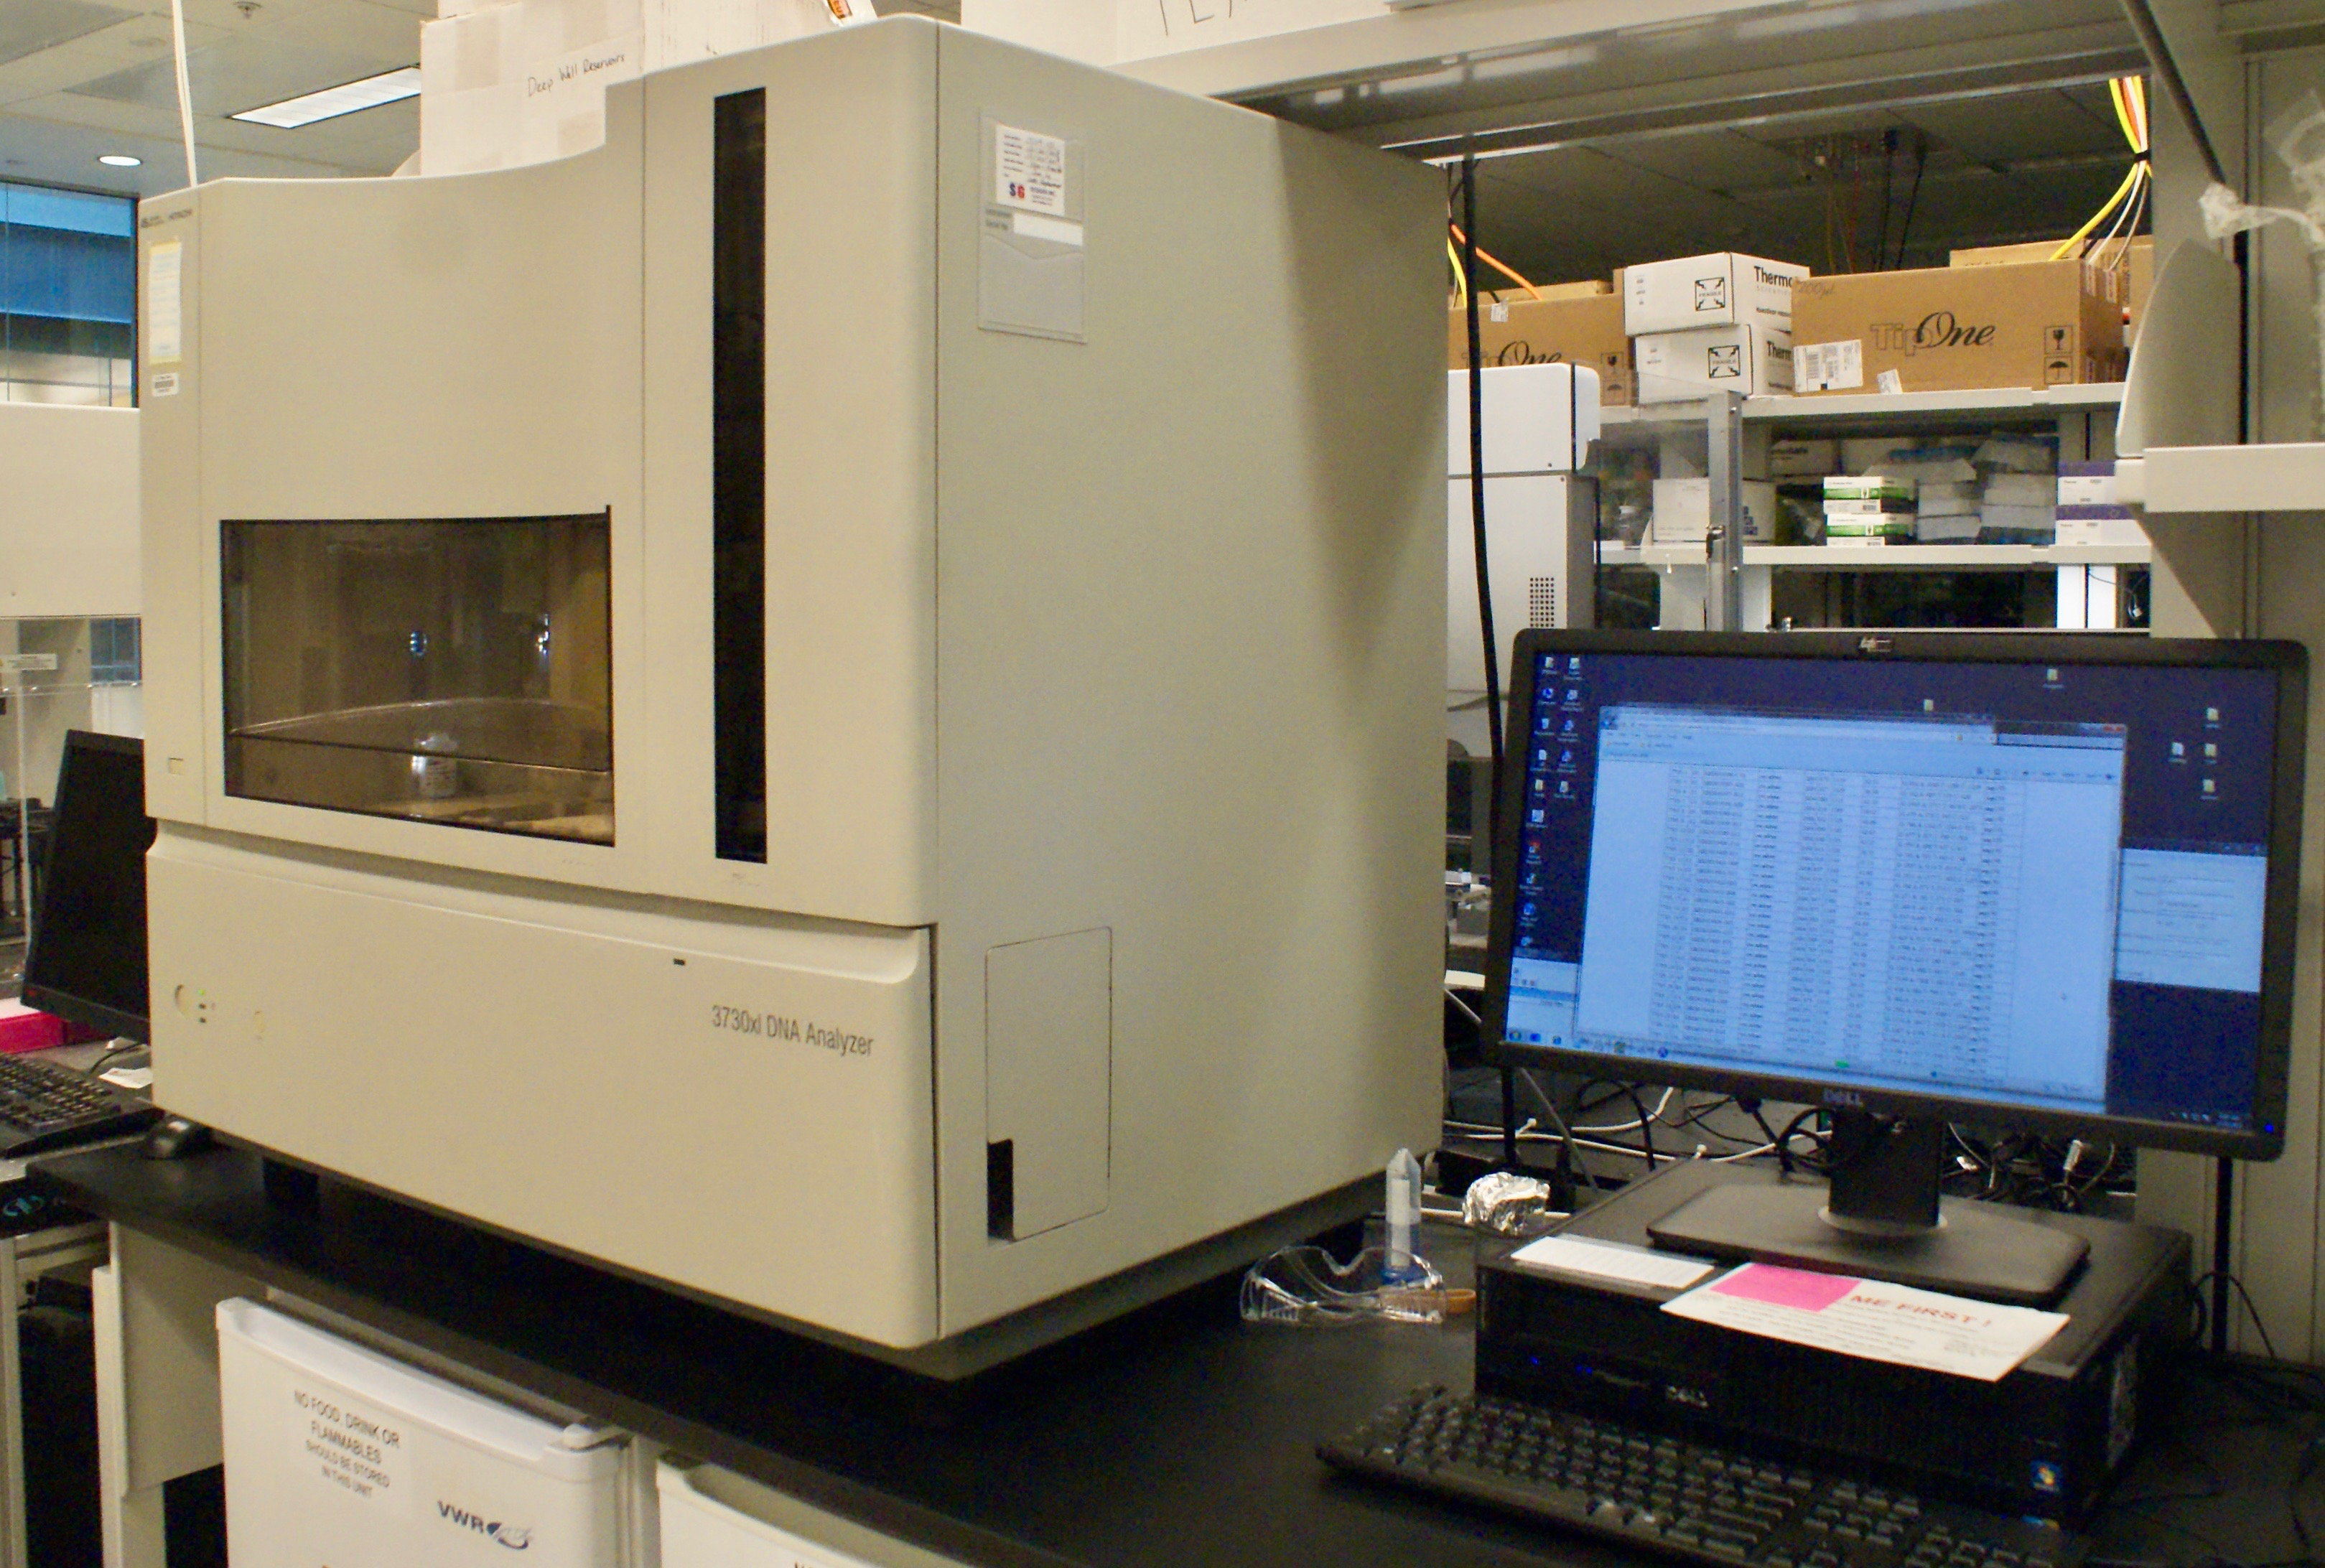
\includegraphics[width=0.7\textwidth]{abi_3730xl_closed.png}
\caption{A closed ABI3730xl capillary electrophoresis DNA analyzer.}
\label{fig:abi_3730xl_closed}
\end{figure}

\begin{figure}[h]
\centering
\includegraphics[width=0.7\textwidth]{abi_3730xl_opened.png}
\caption{An opened ABI3730xl capillary electrophoresis DNA analyzer.}
\label{fig:abi_3730xl_opened}
\end{figure}

\section{Data Structure and Analysis}
\label{sec:data_analysis}

This section explores the structure and organization of the data generated during the DNA sequencing process, which serves as the foundation for the proposed AI-driven tool.

\subsection{Data Collection}

The effectiveness of any artificial intelligence model relies heavily on the quality and structure of the data used for training. In this work, the data originates from customer samples sequenced using the ABI3730xl DNA sequencer. Each well in a 96-well PCR plate generates multiple files, including raw fluorescence data, processed DNA sequences, and quality metrics. With each plate containing 96 wells and each well producing 6 distinct files, a single plate yields 576 files. Over time, as multiple plates are processed daily, this results in millions of files, forming a robust dataset for analysis.
The primary file types considered in this work include:

\begin{itemize}
  \item \textbf{Ab1 File}: Contains intensity readings for each of the four fluorescent dyes (A, T, C, G) used in Sanger sequencing, resulting in fluorescent traces. This file is optimized for long sequences (more than 500 bases).
  \item \textbf{Phd1 File}: Contains the DNA sequence derived from the fluorescence traces, along with quality scores and scan numbers.
  \item \textbf{Scf File}: Similar to .ab1 files, .scf files include quality information about the base calls, the chromatogram (also called the electropherogram), and the DNA sequence.
  \item \textbf{Seq File}: A plain text file containing the DNA sequence.
  \item \textbf{Qual File}: Includes the quality scores of each base in the DNA sequence.
  \item \textbf{Qualtrace File}: Contains additional information about the sequencing process, such as PeakStart, DyeSignal, Noise, and Spacing.
\end{itemize}

These files adhere to a strict naming convention: \textbf{ReactionID\_Pos\_DNAID+PrimerID}. 
For example, the file name \texttt{2338715\_A1\_AA8117+Clon\_2+ORB501} can be broken down as follows:
\begin{itemize}
  \item \texttt{2338715}: The unique reaction ID.
  \item \texttt{A1}: The position of the well in the plate (row A, column 1).
  \item \texttt{AA8117+Clon\_2}: The DNA ID, identifying the specific DNA sample.
  \item \texttt{ORB501}: The primer ID, which is optional as some customers provide samples with primers already included.
\end{itemize}
Thus, 6 files are generated for this specific well: 
\begin{itemize}
  \item \texttt{2338715\_A1\_AA8117+Clon\_2+ORB501.ab1}
  \item \texttt{2338715\_A1\_AA8117+Clon\_2+ORB501.phd.1}
  \item \texttt{2338715\_A1\_AA8117+Clon\_2+ORB501.scf}
  \item \texttt{2338715\_A1\_AA8117+Clon\_2+ORB501.seq}
  \item \texttt{2338715\_A1\_AA8117+Clon\_2+ORB501.qual}
  \item \texttt{2338715\_A1\_AA8117+Clon\_2+ORB501.qualtrace}
\end{itemize}

Other relevant and important information about each plate well, such as the associated \textbf{Client's Name}, and \textbf{Primer DNA Sequence} (If applied by the laboratory staff) is also available.  

\subsection{Database Structure}
For model purposes, the database is structured with only relevant information, and a combination of data that derives from majority of the introduced files coupled with the additional information available.

% section document_structure (end)


